\documentclass[hyperref,UTF8,11pt]{beamer}
\usepackage{ctex}
\usepackage[utf8]{inputenc}
\usepackage{fontspec}
\usepackage{xeCJK}

%-----------------------------------------------------
% Font settings
% 1. For Windows
% \setsansfont{Microsoft YaHei}
% \setCJKmainfont{Microsoft YaHei}
% 2. For macOS
\setCJKmainfont[BoldFont=STSongti-SC-Bold, ItalicFont=STKaitiSC-Regular]{STSongti-SC-Regular}
% This setting is not always valid for your computer.
% You need to configure fonts according to your computer.
%-----------------------------------------------------

\usefonttheme{professionalfonts}
\usepackage{hyperref}
\usepackage{graphicx}
\graphicspath{{figures/}} % storage figure in a sub-folder
% \usepackage[parfill]{parskip} % Activate to begin paragraphs with an empty line rather than an indent
%\usepackage{epstopdf}
\usepackage{bm}
\usepackage{SCUBeamer}
\hypersetup{CJKbookmarks=true}
\usepackage{url}
\usepackage{amsmath}
\usepackage{amsthm}
%\theoremstyle{definition}
%\newtheorem{theorem}{定理}
%\newtheorem{definition}{定义}
%\newtheorem{corollary}{推论}
%\newtheorem{example}{例}
\usepackage{booktabs} % for much better looking tables
%\usepackage{cite} % reference
\usepackage[backend=biber,style=numeric,sorting=none,backref=true]{biblatex}
%\usepackage[backend=biber,style=apalike]{biblatex}
%\usepackage[backend=biber,style=authoryear]{biblatex}
% if style=apalike or authoryear, use \parencite instead of \cite
\addbibresource{references.bib}
\beamertemplatetextbibitems
\usepackage{array} % for better arrays (eg matrices) in maths
%\usepackage{paralist} % very flexible & customisable lists (eg. enumerate/itemize, etc.)
\usepackage{verbatim} % adds environment for commenting out blocks of text & for better verbatim
\usepackage{subfigure} % make it possible to include more than one captioned figure/table in a single float
% These packages are all incorporated in the memoir class to one degree or another...
%\usepackage{threeparttable}
\usepackage{cases} %equation set
\usepackage{multirow} %use table
\usepackage{enumerate}
\usepackage{algorithm}
\usepackage{algorithmic}
\usepackage{xcolor}
%\usepackage{capt-of}
\setcounter{tocdepth}{1}%只显示section,不显示subsection
\usepackage{listings}

\usepackage{calligra}  % 花字体
% \usepackage{setspace}  % 局部调整行距

\lstset{tabsize=4, keepspaces=true,
    xleftmargin=2em,xrightmargin=0em, aboveskip=1em,
    backgroundcolor=\color{gray!20},  % 定义背景颜色
    frame=none,                       % 表示不要边框
    extendedchars=false,              % 解决代码跨页时,章节标题,页眉等汉字不显示的问题
    numberstyle=\ttfamily,
    basicstyle=\ttfamily,
    keywordstyle=\color{blue}\bfseries,
    breakindent=10pt,
    identifierstyle=,                 % nothing happens
    commentstyle=\color{green}\small,  % 注释的设置
    morecomment=[l][\color{green}]{\#},
    numbers=left,stepnumber=1,numberstyle=\scriptsize,
    showstringspaces=false,
    showspaces=false,
    flexiblecolumns=true,
    breaklines=true, breakautoindent=true,breakindent=4em,
    escapeinside={/*@}{@*/},
}

% If your title has two lines, use \\ to wrap
\title[四川大学 Beamer 模板]{四川大学 Beamer 模板}
\subtitle{Beamer Template of Sichuan University}
\author[ShaneTian]{学生:ShaneTian\\ \vskip 4pt 导师:Boss\\ \vskip 4pt 专业:应用统计\\\quad}
\institute[数学学院]{四川大学 \quad 数学学院}
\date{\today}
% \date{2020年6月8日}

\begin{document}
%%%%%%%%%% 定理类环境的定义 %%%%%%%%%%
%% 必须在导入中文环境之后
\newcommand{\redstress}[1]{{\color{scured}{#1}}}
%\renewcommand{\raggedright}{\leftskip=0pt \rightskip=0pt plus 0cm}
\renewcommand{\contentsname}{目录}     % 将Contents改为目录
\renewcommand{\abstractname}{摘要}     % 将Abstract改为摘要
\renewcommand{\refname}{参考文献}      % 将References改为参考文献
\renewcommand{\indexname}{索引}
\renewcommand{\figurename}{图}
\renewcommand{\tablename}{表}
\renewcommand{\appendixname}{附录}
%\renewcommand{\proofname}{证明}
%\renewcommand{\algorithm}{算法}
%----------------------------------------------------------------------
% Title frame
\begin{frame}
\maketitle
\end{frame}

%----------------------------------------------------------------------
% Main frames
%----------------------------------------------------------------------

\section{研究背景与现状}

\begin{frame}{Frame Title}
    \begin{itemize}
        \item My blog: \url{https://suixinblog.cn}
        \item My GitHub: \url{https://github.com/ShaneTian}
        \item My Gitee: \url{https://gitee.com/ShaneTian}
    \end{itemize}
\end{frame}

\begin{frame}{Block}
    \begin{block}{Part 1}
        Test.
    \end{block}
    \begin{theorem}[Thm 1]
        Thm.
    \end{theorem}
    \begin{proof}
        Bingo.
    \end{proof}
\end{frame}

\begin{frame}{Enumerate}
    \begin{equation}
        F=ma\label{Newton2}
    \end{equation}
    \begin{enumerate}
        \item \redstress{BERT~\cite{devlin2018bert}} is a pre-trained model.
        \item Newton's second law of motion \eqref{Newton2}
    \end{enumerate}
\end{frame}


\section{模型与方法}

\begin{frame}{算法}
    \begin{algorithm}[H]
        \caption{算法1}\label{alg:em}
        \begin{algorithmic}[1]
            \REQUIRE Param
            \ENSURE $a$
            \REPEAT
            \STATE Compute $a_n$
            \UNTIL convergence
            \RETURN $a\leftarrow a_n$
        \end{algorithmic}
    \end{algorithm}    
\end{frame}

\begin{frame}{图片}
    \begin{figure}
        \centering
        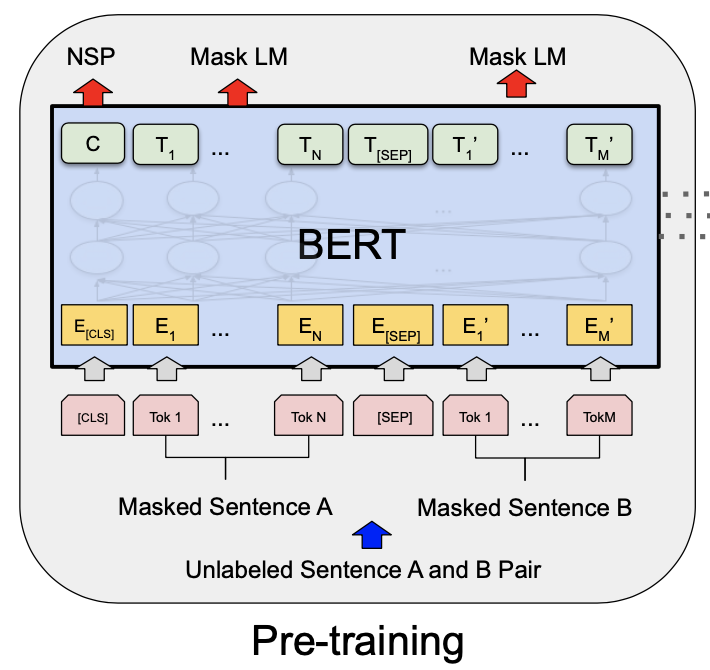
\includegraphics[width=0.5\textwidth]{BERT.png}
        \caption{BERT}\label{fig:bert}
    \end{figure}
\end{frame}

\begin{frame}{分栏}
    \begin{columns}
        \begin{column}{0.5\textwidth}
            \begin{figure}
                \centering
                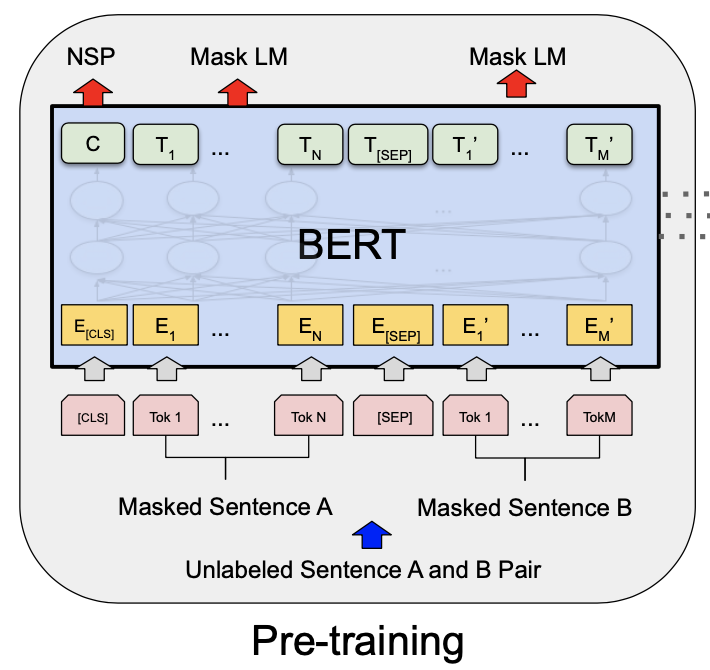
\includegraphics[width=0.95\textwidth]{BERT.png}
                \caption{BERT}\label{fig:bert2}
            \end{figure}
        \end{column}
        \begin{column}{0.5\textwidth}
            \begin{itemize}
                \item Item1
                \item Item2
                \item Item3
                \item ...
            \end{itemize}
        \end{column}
    \end{columns}
\end{frame}

\begin{frame}{Subfigure}
    \begin{figure}
        \centering
        \subfigure[BERT Architecture]{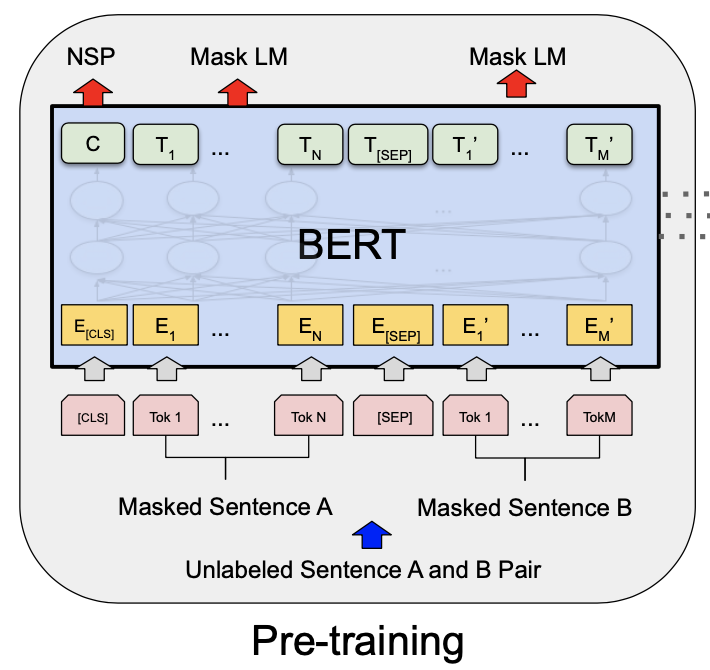
\includegraphics[width=0.4\textwidth]{BERT.png}}
        \hskip 1cm
        \subfigure[SCU logo]{
\includegraphics[width=0.4\textwidth]{SCU.jpeg}}
        \caption{Subfigure\footnote{See: \url{https://github.com/ShaneTian/SCU-Beamer-Template}}}
        \label{fig:subfigure}
    \end{figure}
\end{frame}

% To put the content of a frame in several pages, use allowframebreaks
\begin{frame}[allowframebreaks]
    \frametitle{AllowFrameBreaks}
    \begin{align}
        v&=W_1 x+b_1\label{eq:firstL}\\
        r&=W_2 v+b_2\label{eq:secondL}\\
        \hat{r}&=softmax(r)\label{eq:output}
    \end{align}
    \begin{itemize}
        \item \eqref{eq:firstL} is the first layer.
        \item \eqref{eq:secondL} is the second layer.
        \item \eqref{eq:output} is the output layer.
    \end{itemize}
    \vskip 1cm
    \begin{enumerate}
        \item Item1
        \item Item2
        \item Item3
        \item Item4
        \item Item5
    \end{enumerate}
\end{frame}


\section{实验}

\begin{frame}{More blocks}
    \begin{exampleblock}{Example}
    Eg1.
    \end{exampleblock}
    \begin{alertblock}{Attention}
        Test block!
    \end{alertblock}
\end{frame}

\begin{frame}{表格}
    \begin{table}[]
        {\footnotesize
        \centering
        \caption{实验结果}
        \label{tab:results}
        \begin{tabular}{lcccc}
            \toprule
            \multirow{3}*{\textbf{Model}} & \multicolumn{4}{c}{\textbf{Mean Acc}}\\
            \cmidrule(r){2-5}
            ~ & \multicolumn{2}{c}{\textbf{Dataset1}} & \multicolumn{2}{c}{\textbf{Dataset2}}\\
            ~ & Case1 & Case2 & Case1 & Case2\\
            \midrule
            Model1 & 93.08 & 87.59 & 88.68 & 79.41 \\
            Model2 & 93.14 & 86.67 & 88.41 & 78.66 \\
            Model3 & 92.44 & 87.28 & 87.40 & 78.64 \\
            Model4 & 93.08 & 86.63 & 87.78 & 79.41 \\
            Model5 & \textbf{95.62} & \textbf{91.14} & \textbf{91.96} & \textbf{85.28} \\
            \bottomrule
        \end{tabular}}
    \end{table}
\end{frame}

\begin{frame}[fragile]
    \frametitle{代码}
    \begin{lstlisting}[language=python]
def hello():
    print("Hello World!")
\end{lstlisting}
\end{frame}


\section{总结与展望}

\begin{frame}{总结}
    \begin{description}
        \item[I] First of all
        \item[II] Besides
        \item[III] Last but not least
    \end{description}
\end{frame}

\begin{frame}{展望}
    \begin{description}
        \item[I] First of all
        \item[II] Besides
        \item[III] Last but not least
    \end{description}
\end{frame}

\begin{frame}
    \begin{center}
        \textcolor{scured}{\Huge\calligra Thanks!}
    \end{center}
\end{frame}

\begin{frame}[allowframebreaks]
    \frametitle{参考文献}
    \renewcommand{\bibfont}{\scriptsize}  % 参考文献字体缩小
    \printbibliography
\end{frame}


\end{document}